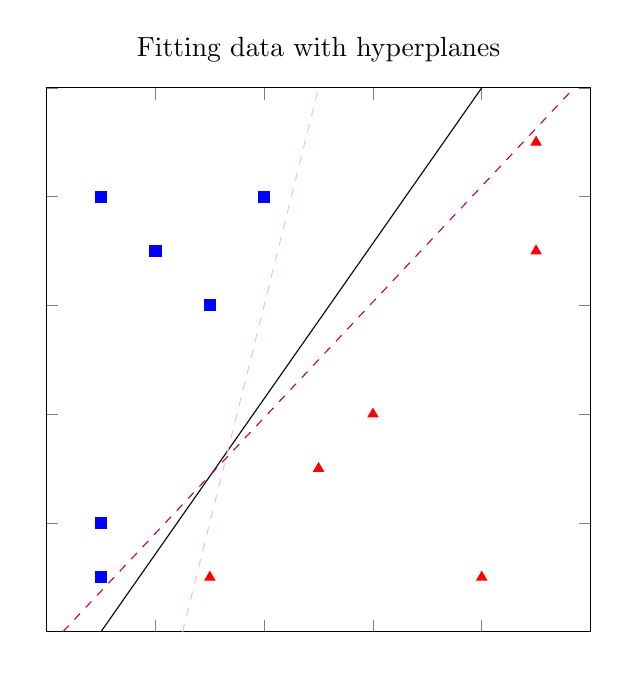
\begin{tikzpicture}
\begin{axis}[
    title={Fitting data with hyperplanes},
    width=.7\textwidth,
    height=.7\textwidth,
    xmin=0, xmax=10,
    ymin=0, ymax=10,
    yticklabels={,,},
    xticklabels={,,},
]
\addplot[
    color=blue,
    mark=square*,
    only marks,
    ]
    coordinates {
    (1,1) (1,2) (1,8) (2,7) (4,8) (3,6)
    };
\addplot[
    color=red,
    mark=triangle*,
    only marks
    ]
    coordinates {
    (3,1) (8,1) (5,3) (6,4) (9,7) (9,9)
    };
\addplot[
    color=black,
    ]
    coordinates{
    (1,0) (8,10)
    };
\addplot[
    color=pink, dashed
    ]
    coordinates{
    (2.5,0) (5,10)
    };
\addplot[
    color=purple, dashed
    ]
    coordinates{
    (0.3,0) (9.7,10)
    };
\end{axis}
\end{tikzpicture}